\part{Strutture dati}

\chapter{Strutture dati fondamentali}
Una struttura dati è un particolare tipo caratterizzato da un modo sistematico di organizzare i dati. Mette a disposizione un insieme di operatori che permettono di memorizzare e manipolare \textit{insiemi dinamici}, cioè insiemi i cui elementi possono variare nel tempo in funzione delle operazioni compiute dall'algoritmo che li utilizza. 

Come vedremo più approfonditamente in seguito, una struttura dati può essere \textit{lineare o non lineare} (a seconda se esista una sequenzializzazione, e se possa essere pensata con un inizio ed una fine), \textit{statica o dinamica} (a seconda che possa variare la sua dimensione nel tempo), \textit{omogenea o disomogenea} (rispetto ai contenuti).

\section*{Insiemi dinamici}
Gli elementi dell'insieme dinamico (spesso chiamati anche \textit{nodi, record, o oggetti}) possono a loro volta essere piuttosto complessi e contenere ciascuno più di un dato “elementare”. In tal caso è abbastanza comune che essi contengano: una \textit{chiave}, utilizzata per distinguere un elemento da un altro, nell’ambito delle operazioni di manipolazione dell'insieme dinamico; \textit{ulteriori dati}, che sono relativi all’elemento stesso ma non sono direttamente utilizzati nelle operazioni di manipolazione. Le tipiche operazioni che si compiono su un insieme dinamico si dividono in due categorie: operazioni di interrogazione (\textit{Search, Minimum, Maximum, Predecessor, Successor}) e operazioni di modifica (\textit{Insert, Delete}).

Le differenti strutture dati che vedremo, se da un lato hanno in comune la capacità di memorizzare insiemi dinamici, dall’altro differiscono anche
profondamente fra loro per le proprietà che le caratterizzano. Sono proprio le proprietà della struttura in questione ad essere l’elemento determinante nella scelta da effettuare quando si deve progettare un algoritmo per risolvere un problema.

Un’ultima considerazione a proposito delle strutture dati è poiché sono destinate alla gestione di insiemi dinamici, è piuttosto comune una loro implementazione mediante l’allocazione dinamica della memoria, per contenerne gli elementi, e l’uso di puntatori, per accedere agli stessi. Alternativamente, possono essere implementate per mezzo di array purché il numero massimo degli elementi possa essere stimato in anticipo.

Prima di studiare alcune strutture dati, da quelle più semplici (\textit{lista, coda e pila}) a quelle più complesse (\textit{albero, grafo}), ne riprendiamo una  che già abbiamo incontrato: l’\textit{array}.

\section{Array}
Innanzitutto, osserviamo che un \textit{array} (sia esso ordinato o no) ha le seguenti caratteristiche: \textit{memorizza elementi omogenei}, cioè dello stesso tipo; \textit{è statico}, cioè ha una lunghezza che deve essere definita a priori; è una struttura ad \textit{accesso casuale}, cioè possiamo accedere ad ogni suo elemento in un tempo costante che è indipendente dalla sua posizione.

Cerchiamo ora di capire quale sia il costo computazionale di alcune delle operazioni sopra citate quando vengano implementate su vettori semplici o ordinati.

\begin{table}[H]
    \centering
    \begin{tabular}{|c|c|c|c|c|c|}
         \hline \textit{Struttura dati} & \textit{Search} & \textit{Min/Max} & \textit{Pre/Succ} & \textit{Insert} & \textit{Delete}\\\hline\hline
         Array qualunque & $O(n)$ & $\Theta(n)$ & $\Theta(n)$ & $\Theta(1)$ & $O(1)$\\\hline
         Array ordinato & $O(\log n)$ & $\Theta(1)$ & $\Theta(1)$ & $O(n)$ & $O(n)$\\\hline
    \end{tabular}
    \caption{Costo computazionale delle operazioni negli array}
    \label{tab:CCArray}
\end{table}

Già da questo semplice confronto si può dedurre come non abbia senso dire che una struttura è migliore di un’altra:
le strutture dati possono essere più o meno adatte ad un certo algoritmo e sta al
buon progettista disegnare un algoritmo efficiente usando la struttura dati più
adatta.

\section{Liste}
Un \textit{puntatore} è una variabile di tipo particolare che contiene l’indirizzo in memoria di un'altra variabile. I puntatori sono necessari per costruire strutture dati dinamiche e per passare i parametri per riferimento. 

La \textit{lista} è una struttura dati nella quale gli elementi sono organizzati in successione. Le proprietà specifiche delle liste sono le seguenti: l’accesso avviene sempre ad una estremità della lista, per mezzo di un’apposita informazione di accesso (puntatore alla testa della lista); è permesso solo un accesso sequenziale agli elementi: non è possibile l’accesso diretto.

A differenza dell'array, la lista può crescere di dimensioni e la successione degli elementi è implementata mediante un collegamento esplicito da un elemento ad un altro. Il valore speciale \verb|None| rappresenta “nessun puntatore” (viene raffigurato con il carattere $\backslash$).
\begin{figure}[H]
    \centering
    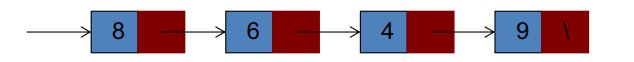
\includegraphics[width=10cm]{images/listaConcatenata.JPG}
    \caption{Lista}
    \label{fig:listaConcatenata}
\end{figure}

\subsection*{Lista puntata semplice}
\begin{wrapfigure}{r}{0.5\textwidth}
 \begin{center}
    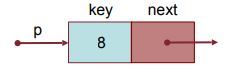
\includegraphics[width=0.48\textwidth]{images/listaConcatenataSingola.JPG}
  \end{center}
\end{wrapfigure}
Ogni elemento di lista è un record a due campi: il campo \textit{key} contiene l’informazione vera e propria; il campo \textit{next} contiene il puntatore che consente l’accesso all’elemento successivo; nel caso dell'ultimo elemento della lista contiene un apposito valore \verb|None| (visualizzato col simbolo $\backslash$). 

\verb|p.key| indica il contenuto del campo key dell'elemento puntato da p. Mentre \verb|p.next| indica il contenuto del campo next dell'elemento puntato da p, ossia l’indirizzo dell'elemento successivo (o None se esso è l’ultimo elemento). 

Ad esempio in Python possiamo definire la classe nodo come segue:
\begin{lstlisting}[language=Python]
    class Nodo:
        def __init__(self, key=None, next=None):
            self.key=key
            self.next=next
\end{lstlisting}
La funzione \verb|Crea| prende in input un array A, genera una lista semplice contenente un nodo per ogni elemento dell'array e termina restituendo la testa alla lista creata. Il costo computazionale della creazione è $\Theta(n)$.
\begin{lstlisting}[language=Python]
    def crea(A):
        if A == []: return None
        p = Nodo(A[0])
        q = p
        for i in range(1,len(A)):
            q.next = Nodo(A[i])
            q = q.next
        return p
\end{lstlisting}
La funzione \verb|Stampa| prende in input il puntatore p alla testa di una lista semplice e stampa i contenuti di ciascun nodo della lista. Il costo computazionale della stampa è $\Theta(n)$.
\begin{lstlisting}[language=Python]     
    def stampa(p):
        while p:
            print(p.key)
            p=p.next
\end{lstlisting}
La funzione \verb|Ricerca|, dato il puntatore p alla testa di una lista semplice e un valore x, restituisce il puntatore al primo nodo della lista contenente il valore x, il puntatore restituito sarà \verb|None| se nella lista un tale nodo non è presente. Il costo computazionale della ricerca è $O(n)$.
\begin{lstlisting}[language=Python]     
    def ricerca(p,x):
        q = p
        while q!=None and q.key != x:
            q = q.next
        return q
\end{lstlisting}

La funzione \verb|Inserisci|, dato il puntatore p alla testa di una lista semplice ed un intero ad un nodo, inserisce un nodo con quel valore in testa alla lista e restituisce la nuova testa della lista. Il costo computazionale dell'inserimento in testa è $\Theta(1)$.
\begin{lstlisting}[language=Python]
    def Inserisci_dopo_q(p,x):
        q = Nodo(x,p)
        return q
\end{lstlisting}

La funzione \verb|Cancella|, dato il puntatore p alla testa di una lista ed il puntatore d ad un nodo della lista
lo cancella e restituisce la testa della lista (eventualmente modificata). Il costo computazionale della cancellazione è $O(n)$.
\begin{lstlisting}[language=Python]
    def cancella(p, d):
        if p == d: return p.next
        q = p
        while q.next != d:
            q = q.next
        q.next = d.next
        return p
\end{lstlisting}

\subsection*{Liste puntata doppia}
Alcuni complicazioni riscontrate nella lista semplice (ad esempio il costo computazionale nella cancellazione) possono essere risolti organizzando la struttura dati in modo che da ogni suo elemento si possa accedere sia all'elemento che lo segue che a quello che lo precede nella lista, quando essi esistono. Tale struttura dati si chiama \textit{lista puntata doppia}.

\begin{figure}[H]
    \centering
    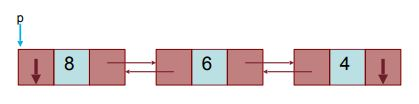
\includegraphics[width=8cm]{images/listeDoppiamentePuntate.JPG}
    \caption{Lista puntata doppia}
    \label{fig:listaDoppPuntata}
\end{figure}

Ad esempio in Python possiamo definire la classe dei nodi di queste liste come:
\begin{lstlisting}[language=Python]
    class NodoD:
        def __init__(self, key=None, prev=None, next=None):
            self.key = key
            self.next = next
            self.prev = prev
\end{lstlisting}
Le operazioni di inserimento e ricerca sono analoghe alle precedenti (con le ovvie modifiche necessarie alla corretta gestione del campo prev). Se voglio “eliminare” dalla lista l’elemento puntato da p:
\begin{lstlisting}[language=Python]
    ...
    p.prev.next = p.next
    p.next.prev = p.prev
    ...
\end{lstlisting}
Il costo computazionale è $\Theta(1)$.

Riassumiamo la situazione nella seguente tabella:
\begin{table}[H]
    \centering
    \begin{tabular}{|c|c|c|c|c|c|}
         \hline \textit{Struttura dati} & \textit{Search} & \textit{Min/Max} & \textit{Pre} & \textit{Insert} & \textit{Delete}\\\hline\hline
         Lista semplice & $O(n)$ & $\Theta(n)$ & $\Theta(n)$ & $\Theta(1)$ & $O(n)$\\\hline
         Lista doppia & $O(n)$ & $\Theta(n)$ & $\Theta(n)$ & $\Theta(1)$ & $\Theta(1)$\\\hline
    \end{tabular}
    \caption{Costo computazionale delle operazioni nelle liste}
    \label{tab:CCListe}
\end{table}

\section{Pile}
\begin{wrapfigure}{r}{0.1\textwidth}
    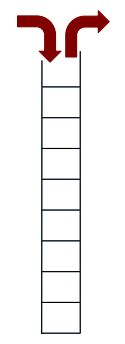
\includegraphics[width=2cm]{images/pila.JPG}
\end{wrapfigure}
La \textit{pila} è una struttura dati che esibisce un comportamento \textit{LIFO} (Last In First Out). In altre parole, la pila ha la proprietà che gli elementi vengono prelevati dalla pila nell’ordine inverso rispetto a quello col quale vi sono stati inseriti.

Su una pila sono definite solo due operazioni: l’inserimento (che di norma viene chiamata \textit{Push}) e l’estrazione (che di norma viene chiamata \textit{Pop}). La particolarità che garantisce la proprietà LIFO è che le operazioni Push e Pop operano sulla stessa estremità della pila (attraverso il puntatore \textit{top}).

\subsubsection{Implementazione con liste puntate}
La funzione \verb|Push| riceve il puntatore alla cima della pila ed il valore da inserire, lo inserisce in un nodo in cima alla lista puntata e restituisce la nuova cima.
\begin{lstlisting}[language=Python]
    def push(top, x):
        top = Nodo(x,top)
        return top
\end{lstlisting}

La funzione \verb|Pop| prende il puntatore alla cima della pila e restituisce il valore del nodo in cima alla pila e la nuova cima della pila.
\begin{lstlisting}[language=Python]
    def pop(top):
        if top == None:
            print('Errore pila vuota')
            return None, None
        return top.key, top.next
\end{lstlisting}

\subsubsection{Implementazione con liste}
\begin{lstlisting}[language=Python]
    def push(Pila, x):
        Pila.append(x)
        
    def pop(Pila):
        if Pila == []: return None
        return Pila.pop()
\end{lstlisting}

Per entrambe le implementazioni (liste o liste puntate) il costo computazionale di Push e Pop, è $\Theta(1)$.


\section{Code}
La \textit{coda} è una struttura dati che esibisce un comportamento \textit{FIFO} (First In First Out). In altre parole, la coda ha la seguente proprietà: gli elementi vengono prelevati dalla coda esattamente nello stesso ordine col quale vi sono stati inseriti.

Su una coda sono definite solo due operazioni: l’inserimento (che di norma viene chiamata \textit{Enqueue}) e l’estrazione (che di norma viene chiamata \textit{Dequeue}). Viceversa, di solito non si scandiscono gli elementi di una coda né si eliminano elementi con mezzi diversi dalla Dequeue. La particolarità che garantisce la proprietà FIFO è che l’operazione Enqueue opera su una estremità della coda (\textit{tail}) e la Dequeue opera sull’altra estremità (\textit{head}):

\begin{figure}[H]
    \centering
    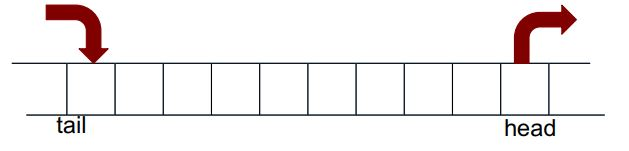
\includegraphics[width=8cm]{images/coda.JPG}
    \caption{Rappresentazione di una coda}
    \label{fig:coda}
\end{figure}

\subsubsection{Implementazione con liste puntate}
La funzione \verb|Enqueue| prende in input i puntatori alla testa e alla coda ed il valore da inserire e dopo aver inserito il nodo col nuovo valore in coda restituisce i puntatori alla testa ed alla coda.
\begin{lstlisting}[language=Python]
    def inserisci(testa, coda, x):
        e = Nodo(x)
        if testa == None: return e, e
        coda.next = e
        return testa, e
\end{lstlisting}

La funzione \verb|Dequeue| prende in input i puntatori alla testa e alla coda e dopo aver estratto il valore del nodo in testa lo restituisce con i puntatori alla testa ed alla coda.
\begin{lstlisting}[language=Python]
    def estrai(testa, coda):
        if testa == None: 
            print('Errore: coda vuota')
            return None, None, None
        if testa == coda:
            return testa.key, None, None
        return testa.key, testa.next, coda
\end{lstlisting}

\subsubsection{Implementazione con liste}
\begin{lstlisting}[language=Python]
    def inserisci(Coda, testa, x):
        Coda.append(x)
        if testa == None: return 0
        return testa
    
    def estrai(Coda, testa):
        if testa == len(Coda):
            print('Errore coda vuota')
            return None, testa
        return Coda[testa], testa+1
\end{lstlisting}

Per entrambe le implementazioni (liste o liste puntate) il costo computazionale di Push e Pop, è $\Theta(1)$.

\section{Alberi}
Un \textit{albero} è una struttura dati estremamente versatile, utile per modellare una grande quantità di situazioni reali e progettare le relative
soluzioni algoritmiche.

\subsection*{Alberi radicati}
In un \textit{albero radicato}: i nodi sono organizzati in livelli, numerati in ordine crescente allontanandosi dalla radice (di norma la radice è posta a
livello zero); l’altezza di un albero radicato è la lunghezza del più lungo cammino dalla radice ad una foglia; un albero di altezza h contiene h+1 livelli, di norma numerati da ad 0 ad h.
\begin{figure}[H]
    \centering
    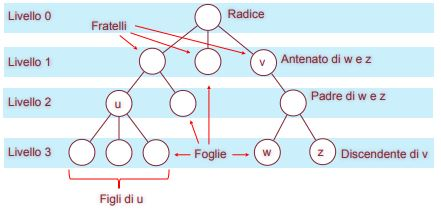
\includegraphics[width = 10cm]{images/esempioAlberoRadicato.JPG}
    \caption{Albero radicato}
    \label{fig:esAlberoRadicato}
\end{figure}
Un albero radicato si dice ordinato se attribuiamo un qualche ordine ai figli di ciascun nodo, nel senso che se un nodo ha k figli, allora vi è un figlio che viene considerato primo, uno che viene considerato secondo, ..., uno che viene considerato k-esimo.

Una particolare sottoclasse di alberi radicati e ordinati è quella degli alberi binari.

\subsection*{Alberi binari}
Gli \textit{alberi binari} hanno la particolarità che ogni nodo ha al più due figli. Poiché sono alberi ordinati, i due figli di ciascun nodo si distinguono in \textit{figlio sinistro} e \textit{figlio destro}. Un albero binario nel quale tutti i livelli contengono il massimo numero possibile di nodi è chiamato \textit{albero binario completo}. Se invece tutti i livelli tranne l’ultimo contengono il massimo numero possibile di nodi, l’albero è chiamato \textit{albero binario quasi completo}.
\begin{figure}
    \centering
    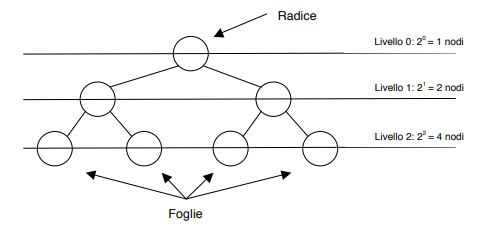
\includegraphics[width = 10cm]{images/alberoBinarioCompleto.JPG}
    \caption{Albero binario}
    \label{fig:alberoBinarioCompleto}
\end{figure}

Il numero delle foglie di un albero binario è $2^h$; il numero dei nodi interni è $\sum^{h-1}_{i=0}2^i=\frac{2^h-1}{2-1}=2^h-1$; il numero totale dei nodi è $2^h+2^h-1=2^{h+1}-1$.
In ultima analisi l'altezza h di un albero binario completo è dato dal numero dei nodi $n=2^{h+1}-1$ da cui segue che $\log_2(n+1)=h+1$ e quindi:
\begin{equation*}
    h = \log_2(n+1)-1 = \log_2\frac{n+1}{2}\hspace{1cm}h=\Theta(\log n)
\end{equation*}
In generale per un albero binario si ha $\Omega(\log n)=h\leq n-1$.

\subsubsection{Rappresentazione di un albero binario}
Il modo più naturale di rappresentare e gestire gli alberi binari è per mezzo dei puntatori. Ogni singolo nodo è costituito da un record contenente: \textit{key}: le opportune informazioni pertinenti al nodo stesso; \textit{left}: il puntatore al figlio sinistro (oppure \verb|None| se il nodo non ha figlio sinistro); \textit{right}: il puntatore al figlio destro (oppure \verb|None| se il nodo non ha figlio destro).\\
Si accede all’albero per mezzo del puntatore alla radice.

\begin{figure}[H]
    \centering
    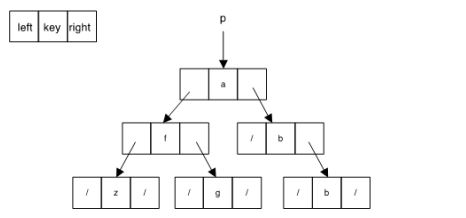
\includegraphics[width = 10cm]{images/rappresentazioneAlbero.JPG}
    \caption{Albero binario con puntatori}
    \label{fig:rappAlberoBin}
\end{figure}

Questo tipo di memorizzazione ha tutti i vantaggi e l’elasticità delle strutture dinamiche basate sui puntatori (si possono inserire nuovi nodi, spostare dei nodi ecc.). In una struttura di questo tipo il codice per la creazione di ogni nodo dell'albero è il seguente:
\begin{lstlisting}[language=Python]
    class NodoAB:
        def __init__(struct, key=None, fs=None, fd=None):
            struct.key = key
            struct.fs = fs
            struct.fd = fd
\end{lstlisting}
Ora abbiamo tutto il necessario per creare un albero binario random (dove $n$ rappresenta il numero di nodi e $m$ il valore delle chiavi di ogni singolo nodo in un intervallo $[0,m]$ ):
\begin{lstlisting}[language=Python]
    import random
    def crea(n, m):
        if n == 0: return None
        r = NodoAB(random.randint(0,m))
        s = random.randint(0,n-1)
        r.fs = crea(s, m)
        r.fd = crea(n-s-1, m)
        return r
\end{lstlisting}

\subsubsection{Visita in un albero binario}
Un’operazione basilare sugli alberi, che spesso è il presupposto per poter risolvere problemi su di essi, è l’accesso a tutti i suoi nodi, uno dopo l’altro, al fine di poter effettuare una specifica operazione (che dipende ovviamente dal problema posto) su ciascun nodo. Abbiamo visto come tale operazione sulle liste sia una semplice iterazione, ma sugli alberi la situazione è più complessa dato che la loro struttura è ben più articolata.

L’accesso progressivo a tutti i nodi di un albero si chiama \textit{visita dell'albero}. Facendo riferimento all’ordine col quale si accede ai nodi dell'albero, è evidente che esiste più di una possibilità.
Nel caso specifico degli alberi binari, nei quali i figli di ogni nodo (e quindi i sottoalberi) sono al massimo due, e volendo comportarsi nello stesso modo su tutti i nodi, le possibili decisioni in merito a questa scelta danno luogo a tre diverse visite: 
\begin{itemize}
    \item \textit{preorder}: il nodo è visitato prima di proseguire la visita nei suoi sottoalberi;
    \item \textit{inorder}: il nodo è visitato dopo la visita del sottoalbero sinistro e prima di quella del sottoalbero destro;
    \item \textit{postorder}: il nodo è visitato dopo entrambe le visite dei sottoalberi.
\end{itemize}

Con le nozioni apprese possiamo risolvere dei semplici ma utili problemi sugli alberi.
\begin{enumerate}
    \item Dato il puntatore alla radice stampare un albero binario di n nodi:
    \begin{lstlisting}[language=Python]
        def stampa(r):
            if r == None: return
            print(r.key)
            stampa(r.fs)
            stampa(r.fd)
    \end{lstlisting}
    
    \item Dato il puntatore alla radice calcolare il numero di nodi di un albero:
    \begin{lstlisting}[language=Python]
        def conta(r):
            if r == None: return 0
            return 1 + conta(r.fs) + conta(r.fd)
    \end{lstlisting}
    
    \item Dato il puntatore alla radice calcolare l'altezza dell'albero:
    \begin{lstlisting}[language=Python]
        def altezza(r):
            if r == None: return 0
            a = altezza(r.fs)
            b = altezza(r.fd)
            return max(a,b) + 1
    \end{lstlisting}
\end{enumerate}


\chapter{Dizionari}
Un dizionario è una struttura dati che permette di gestire un insieme dinamico di dati tramite queste tre sole operazioni:
\begin{itemize}
    \item \verb|insert|: si inserisce un elemento;
    \item \verb|search|: si ricerca un elemento;
    \item \verb|delete|: si elimina un elemento.
\end{itemize}

\section{Tablelle Hash}
Una \textit{tabella hash} (in inglese hash table) è una struttura di dati efficiente per implementare dizionari. Sotto ragionevoli assunzioni, le tabelle hash implementano le tre operazioni di inserimento, cancellazione e ricerca con complessità media costante $\Theta(1)$.

Per implementare una tabella hash bisogna dimensionare la tabella in base al numero di elementi attesi (che indicheremo con m) ed  utilizzare una speciale funzione (funzione hash) per indicizzare la tabella.

\subsection*{Funzione Hash}
Una \textit{funzione hash} è una funzione che data una chiave x restituisce la posizione della tabella in cui l’elemento con
chiave x viene memorizzato: $h(x)\in\{0,1,...,m-1\}$.
La dimensione m della tabella può non coincidere con l'insieme degli elementi n, anzi in generale $m<<n$.

L’idea è quella di definire una funzione d’accesso che permetta di ottenere la posizione di un elemento data la sua chiave in questo modo riduciamo lo spazio necessario per memorizzare la tabella ma perdiamo la corrispondenza tra chiavi e posizioni in tabella. Inoltre le tabelle hash possono soffrire del fenomeno delle collisioni, dato che il numero di posizioni è molto minore a quello degli elementi da inserire, capiterà che la funzione restituisca lo stesso valore per entrambe le chiavi, che quindi andrebbero memorizzate nella stessa posizione della tabella. 

Una buona funzione hash dovrà essere in grado di distribuire uniformemente le chiavi nello spazio degli indici. La situazione ideale è quella in cui ciascuna delle m posizioni della tabella è scelta con la stessa probabilità.

Un metodo semplicissimo per definire una funzione hash è dello del modulo: $h(k)=k \mod m$. Nella maggior parte dei casi questo metodo da buoni risultati ma vi sono situazioni in cui si può essere particolarmente sfortunati. Pertanto, nei successivi paragrafi, illustreremo i due metodi più diffusi per la gestione delle collisioni (indirizzamenti chiusi e aperti).

\subsection*{Indirizzamento chiuso}
In un'\textit{indirizzamento chiuso} ad ogni cella della tabella hash si fa corrispondere una lista (solitamente una lista concatenata) detta \textit{lista di trabocco}. In questo modo un elemento che collide viene aggiunto alla lista corrispondente all'indice ottenuto.
\begin{figure}[H]
    \centering
    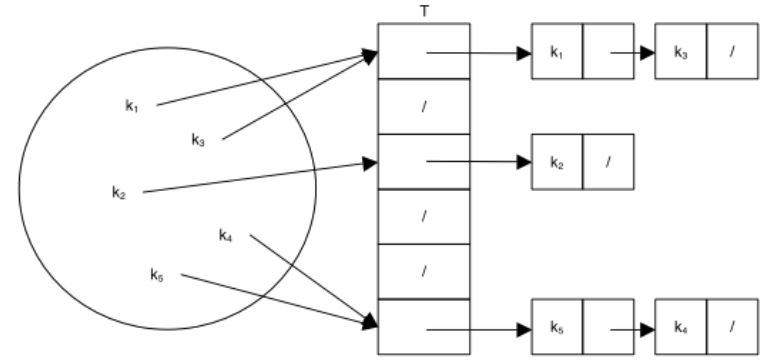
\includegraphics[width=10cm]{images/indirizzamento_chiuso.JPG}
    \caption{Indirizzamento chiuso con liste di trabocco}
    \label{fig:indirizzamento_chiuso}
\end{figure}

Analizziamo ora le principali operazioni da compiere:
\begin{itemize}
    \item L'\textit{inserimento} avviene in $\Theta(1)$, essendo una lista a puntatori si può sempre inserire in tempo costante in testa alla lista;
    \item Nella \textit{ricerca} il caso pessimo si verifica quando tutti gli elementi memorizzati nella tabella hash mappano alla medesima posizione generando una complessità dell'ordine $O(n)$. Nel caso medio, invece, (quando la funzione hash gode di uniformità semplice) è $O(1+\frac{n}{m})=O(1+\alpha)$ dove con $\alpha$ indichiamo il fattore di carico della tabella;
    \item Per la \textit{cancellazione} infine dipende dall'implementazione delle liste di trabocco e valgono, pertanto, tutte le osservazioni fatte per il costo dell'operazione di cancellazione nelle liste.
 
\end{itemize}

\subsection*{Indirizzamento aperto}
L'\textit{indirizzamento aperto} prevede di inserire tutti gli elementi direttamente nella tabella, senza far uso di strutture dati aggiuntive. Essa è applicabile quando: $n\leq m$ quindi il fattore di carico ($\frac{n}{m}$) è $\alpha<1$.

Supponiamo di voler inserire una chiave k e che la sua posizione “naturale” $h(k)$ sia già occupata. L’indirizzamento aperto consiste nell’occupare un’altra cella vuota, anche se essa potrebbe spettare di diritto ad un’altra chiave. Se la posizione iniziale relativa alla chiave k è occupata, si scandisce la tabella fino a trovare una posizione libera nella quale l’elemento con chiave k può essere memorizzato. 

\begin{figure}[H]
    \centering
    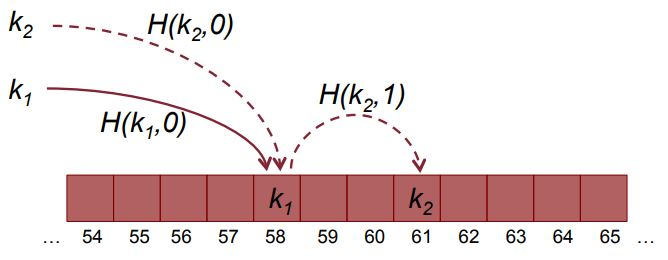
\includegraphics[width = 12cm]{images/indirizzamento_aperto.JPG}
    \caption{Indirizzamento aperto}
    \label{fig:indirizzamento_aperto}
\end{figure}

Anche in questo caso analizziamo il costo delle operazioni:
\begin{itemize}
    \item Per l'\textit{inserimento}, quando si incontra una collisione, non si fa altro che utilizzare l’indice successivo a quello che collide sino a che non si trovi una casella libera. Oppure si utilizza un'ulteriore funzione hash in modo tale che, se le due funzioni sono ben progettate, è estremamente improbabile che due chiavi $k_1$ e $k_2$ producano una collisione su entrambe le funzioni hash;
    \item L’operazione di \textit{ricerca} è simile a quella di inserimento. Se durante la scansione delle celle viene trovata una cella che contiene la chiave l’operazione restituisce l’elemento trovato. Se invece si arriva ad una cella vuota o si è scandita senza successo tutta la tabella si restituisce \verb|None|. 
    \item Per la \textit{cancellazione} la prima cosa che verrebbe in mente è quella di eliminare con la cella dell'array che contiene la chiave. Così facendo la ricerca non sarebbe più corretta infatti potrebbe interrompersi prima di trovare l’elemento cercato per via di un “buco” creato dalla cancellazione (in pratica potrebbe accadere che un elemento presente in tabella non venga trovato). Quindi marchiamo le celle che hanno subito cancellazione con un valore speciale \verb|canc|.
\end{itemize}

\section{Alberi binari di ricerca}
Gli \textit{alberi binari di ricerca} (ABR) sono alberi binari nei quali vengono mantenute le seguenti proprietà:
\begin{itemize}
    \item ogni nodo dell'albero contiene una chiave; 
    \item il valore della chiave contenuta in ogni nodo è maggiore al valore della chiave contenuta in ciascun nodo del suo sottalbero sinistro (se esso esiste);
    \item il valore della chiave contenuta in ogni nodo è minore al valore della chiave contenuta in ciascun nodo del suo sottalbero destro (se esso esiste).
\end{itemize}

\begin{figure}[H]
    \centering
    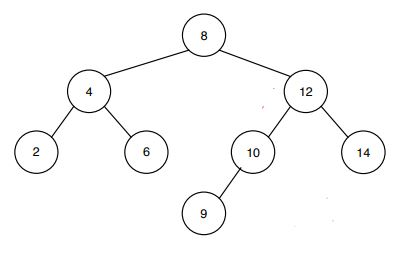
\includegraphics[width = 8cm]{images/alberi_di_ricerca.JPG}
    \caption{Albero binaro di ricerca}
    \label{fig:alberi_ricerca}
\end{figure}

Per inciso in un ABR il minimo è sempre nel nodo più a sinistra, il massimo in quello più a destra. Si noti che il nodo più a sinistra non necessariamente è una foglia; analoga considerazione per il nodo più a destra.

\subsubsection{Ricerca su un albero binario di ricerca}
Il procedimento di ricerca su un ABR è concettualmente simile alla ricerca binaria ed è molto semplice: si esegue una discesa dalla radice che viene guidata dai valori memorizzati nei nodi che si incontrano lungo il cammino. Quando si trova in un nodo il valore ricercato si termina con successo restituendo il puntatore al nodo. Se invece si arriva ad una foglia che non lo contiene si termina senza successo restituendo \verb|Null|.
\begin{lstlisting}[language=Python]
    def ricercaABR(p,x):
        if p == None or p.key == x:
            return p
        if p.key < x:
            return ricercaABR(p.right, x)
        return ricercaABR(p.left, x)
\end{lstlisting}
Per quanto riguarda il costo computazionale della funzione di ricerca, intuitivamente, dato che la ricerca percorre un singolo cammino dalla radice ad una foglia, ci aspettiamo che esso sia legato all’altezza h dell'albero.
\begin{equation*}
    T(h)=O(h)
\end{equation*}

Come mai non riusciamo a garantire un costo logaritmico per la ricerca come per gli alberi binari? La ragione risiede nel fatto che l'ABR non include fra le sue proprietà alcuna relazione con la sua altezza, infatti sono alberi binari di ricerca anche alberi con un solo ramo lungo h.

\subsubsection{Inserimento in un albero binario di ricerca}
Anche il procedimento di inserimento su un ABR è molto semplice: si esegue una discesa che, come nel caso della ricerca, viene guidata dai valori memorizzati nei nodi che si incontrano lungo il cammino. Quando si arriva al punto di voler proseguire la discesa verso un puntatore vuoto (\verb|Null|) allora, in quella posizione, si aggiunge un nuovo nodo contenente il valore da inserire.

In realtà il metodo più efficiente consiste nell'aggiunta di un nuovo campo ai nodi dell'albero in cui viene memorizzato il puntatore al padre (\verb|parent|).

\subsubsection{Massimo e minimo in un albero binario di ricerca}
Il \textit{minimo} (\textit{massimo}) si trova nel nodo più a sinistra (destra), quindi per trovarlo si scende sempre a sinistra (destra) a partire dalla radice. Ci si ferma quando si arriva a un nodo che non ha figlio sinistro (destro): quel nodo contiene il minimo (massimo).

\subsubsection{Predecessore e successore in un albero binario di ricerca}
Per \textit{predecessore} di k si intende il nodo dell'albero contenente la chiave che precederebbe immediatamente k se le chiavi fossero ordinate. Notiamo come se il nodo che contiene k ha il sotto-albero sinistro, il suo predecessore è il massimo di tale sotto-albero. Mentre se il nodo che contiene k non ha sotto-albero sinistro vuol dire che esso è il nodo più a sinistra di un certo sotto-albero. Per trovare il suo predecessore bisogna risalire alla radice di quel sotto-albero, il che significa salire a destra finché è possibile e una volta giunti nella radice del sotto-albero, si risale (con un singolo passo di salita a sinistra) a suo padre che è il predecessore di k. 

Una situazione perfettamente simmetrica esiste per il problema di trovare il \textit{successore} di un nodo, dove per successore si intende il nodo che contiene la chiave che seguirebbe immediatamente k se le chiavi fossero ordinate.


\subsubsection{Cancellazione in un albero binario di ricerca}
Il problema di eliminare una chiave contenuta in un ABR è il più complicato, poichè si possono verificare vari casi in base al numero di figli del nodo che si vuole cancellare:
\begin{itemize}
    \item se il nodo è una foglia lo si elimina, ponendo a NULL l’opportuno campo nel nodo padre $\Theta(1)$;
    \item se il nodo ha un solo figlio si collegano direttamente fra loro suo padre e il suo unico figlio, indipendentemente che sia destro o sinistro $\Theta(1)$;
    \item se il nodo ha entrambi i figli lo si sostituisce con il massimo contenuto nei suoi sotto-alberi. A sua volta il massimo va eliminato dalla sua posizione originale. Si noti che, per trovare il massimo si cercherà sempre nel sotto-albero destro e per cancellarlo si userà sicuramente il caso 1 o il caso 2, infatti il massimo non può avere il figlio destro perchè altrimenti non sarebbe lui il massimo (il figlio destro avrebbe un valore maggiore di quello del padre) $O(h)$;
\end{itemize}


\section{Alberi di ricerca bilanciati}
Come abbiamo visto, un ABR di altezza h contenente n nodi supporta le operazioni fondamentali dei dizionari in tempo $O(h)$, ma purtroppo non si può escludere che h sia $O(n)$, con conseguente degrado delle prestazioni. Viceversa, tutte le operazioni restano efficienti se si riesce a garantire che l’altezza dell'albero sia piccola, in particolare sia $O(\log n)$.

Per raggiungere tale scopo esistono varie tecniche, dette di \textit{bilanciamento}, tutte basate sull'idea di riorganizzare la struttura dell'albero se essa, a seguito di un'operazione di inserimento o di eliminazione di un nodo, viola determinati requisiti. In particolare, il requisito da controllare è che, per ciascun nodo dell'albero, l’altezza dei suoi due sotto-alberi non sia “troppo differente”. Ciò che rende non banali queste tecniche è che si vuole aggiungere agli alberi di ricerca una proprietà (il bilanciamento) senza peggiorare il costo computazionale delle operazioni.

\subsection*{Alberi red-black}
Illustreremo ora una di tali tecniche, quella degli RB-alberi (\textit{alberi Red-Black}).

Un RB-albero è un ABR i cui nodi hanno un campo aggiuntivo, il colore, che può essere solo rosso o nero. Alla struttura si aggiungono foglie fittizie (che non contengono chiavi) per fare in modo che tutti i nodi “veri” dell'albero abbiano esattamente due figli.

Un RB-albero è un ABR che soddisfa le seguenti proprietà aggiuntive:
\begin{enumerate}
    \item ciascun nodo è rosso o nero;
    \item ciascuna foglia fittizia è nera;
    \item se un nodo è rosso i suoi figli sono entrambi neri;
    \item ogni cammino da un nodo a ciascuna delle foglie del suo sotto-albero contiene lo stesso numero di nodi neri.
\end{enumerate}

Col termine b-altezza di x (black height di x, $bh(x)$) si indica il numero di nodi neri sui cammini dal nodo x alle foglie sue discendenti. La b-altezza di un RB-albero è la b-altezza della sua radice.

\begin{figure}
    \centering
    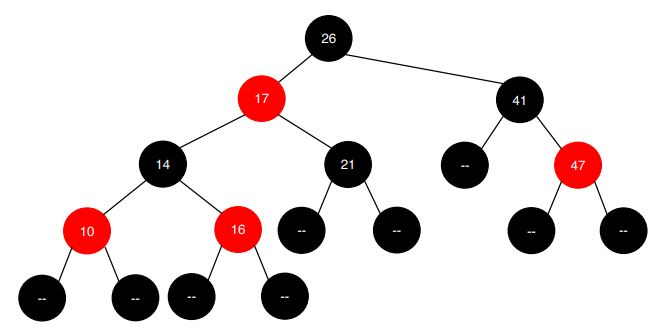
\includegraphics[width = 12cm]{images/rb-albero.JPG}
    \caption{Albero red-black}
    \label{fig:rb_albero}
\end{figure}

Dalla combinazione delle proprietà 3 e 4 discende un fatto interessante: nessun cammino dalla radice ad una foglia può essere lungo più del doppio di un cammino dalla radice ad una qualunque altra. Questo perché il numero di nodi neri è il medesimo lungo tutti i cammini (proprietà 4) e il numero di nodi rossi lungo un cammino non può essere maggiore del numero di nodi neri lungo lo stesso cammino (proprietà 3). Quindi un cammino che contiene il massimo numero possibile di nodi rossi non può essere lungo più del doppio di un cammino composto solo di nodi neri. Questa proprietà è sufficiente a dimostrare che l’altezza di un RB-albero di n nodi è $O(\log n)$.

Questa proprietà ci garantisce che le operazioni di ricerca di una chiave, del massimo o del minimo, del predecessore o del successore, siano tutte eseguite con un costo computazionale $O(\log n)$. Discorso a parte va fatto invece per gli inserimenti e le cancellazioni. Infatti, l’esigenza di mantenere le proprietà di RB-albero implica che, dopo un inserimento o una cancellazione, la struttura dell'albero possa dover essere riaggiustata, in termini di: colori assegnati ai nodi o struttura dei puntatori (ossia, collocazione dei nodi nell'albero).

A tal fine sono definite apposite operazioni, dette \textit{rotazioni}, che permettono di ripristinare in tempo $O(\log n)$ le proprietà del RB-albero dopo un inserimento o un’eliminazione. Le rotazioni, che possono essere destre o sinistre, sono operazioni locali che non modificano l’ordinamento delle chiavi secondo la visita in-ordine, e possono essere schematizzate come riportato nella figura seguente:
\begin{figure}[H]
    \centering
    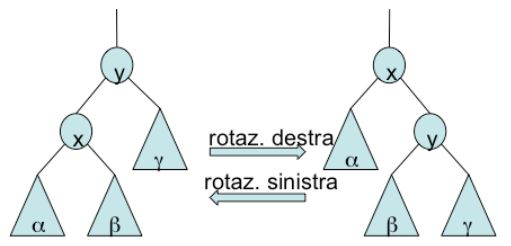
\includegraphics[width = 8cm]{images/rotazioni-rb.JPG}
    \caption{Rotazioni destre e sinistre di un albero red-black}
    \label{fig:dx_sx_redblack}
\end{figure}

Possiamo osservare che effettuare ciascuna rotazione implica un costo costante poiché coinvolge un numero costante di puntatori, essendo
un’operazione locale.

\begin{lstlisting}[language=Python]
    def RBA_rotaz_sinistra(p, a):
        b = a.right
        a.right = b.left
        if b.left!= None:
            b.left.parent = a
        b.left = a
        b.parent = a.parent
        if a == p:
            p = b
        elif a==a.parent.left:
            a.parent.left = b
        else:
            a.parent.right = b
        a.parent = b
        return p
\end{lstlisting}
Lo codice della rotazione a destra è analogo.

Possiamo ora descrivere l’algoritmo di inserimento di una chiave in un albero red-black. Si utilizza l’algoritmo di inserimento in un ABR, colorando il nodo sempre di rosso. L'unica regola che può essere infranta è la 3 (entrambi i figli di un nodo rosso sono neri), infatti il nuovo nodo (rosso) potrebbe essere inserito come figlio di un nodo rosso.

Dobbiamo dunque procedere ad aggiustare la struttura solo in questo caso. Si presentano 3 possibili eventualità da gestire in modo diverso:
\begin{enumerate}
    \item Il nodo inserito è figlio di un nodo rosso e lo zio è rosso;
    \item Il nodo inserito è figlio destro di un nodo rosso e lo zio è nero;
    \item Il nodo inserito è figlio sinistro di un nodo rosso e lo zio è nero.
\end{enumerate}

Per il primo caso si cambiano i colori di alcuni nodi: detto x il nuovo nodo appena inserito, si colorano di nero il padre e lo zio di x, di rosso il nonno di x. A questo punto, o la violazione è stata eliminata o è stata portata più in alto, e si ripresenta di nuovo.
Per il secondo caso  si effettua una rotazione a sinistra imperniata sul padre di x, e questo conduce sempre al terzo caso.
Per il terzo caso si effettua una rotazione a destra e ed eventualmente si cambiano i colori dei figli, il che garantisce sempre la soluzione della violazione.

Ne consegue che, durante un inserimento, è possibile entrare più volte nel caso 1, eventualmente nel caso 2, e si conclude sempre con il caso 3.
Poiché ogni volta che si presenta un nuovo caso da risolvere, la violazione si è spostata più in alto, avremo al più $O(\log n)$ iterazioni di costo costante, provando così che in un albero red-black si può inserire una nuova chiave in tempo $O(\log n)$.

Lo stesso vale per la cancellazione.

\begin{figure}
    \centering
    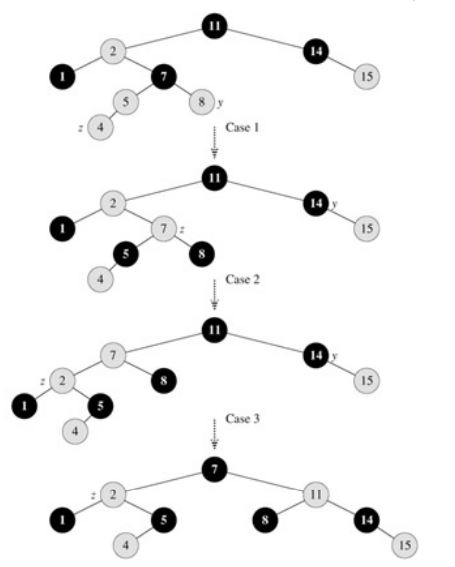
\includegraphics[width = 10cm]{images/case-rb.JPG}
    \caption{Casi in uso per gli alberi red-black}
    \label{fig:case-rb}
\end{figure}



\chapter*{Esercizi svolti}
\addcontentsline{toc}{chapter}{Esercizi svolti}
\begin{exercise}[Liste]\phantom{}
\begin{itemize}
    \item Dato il puntatore di una lista, scrivere una funzione che in tempo $\Theta(n)$ restituisce la lista invertita. Il programma non deve generare nuovi nodi ma lavorare sui nodi della lista originaria.
    \begin{lstlisting}[language=Python]
        def inverti(p):
            q = None
            while p != None:
                s = p
                p = p.next
                s.next = q
                q = s
            return q
    \end{lstlisting}
    
    \item Dato il puntatore di una lista ordinata ed un intero x scrivere una funzione che in tempo $\Theta(n)$ inserisce un nodo con chiave x nella lista in modo che questa risulti ancora ordinata in modo crescente e restituisce il puntatore alla lista.
    \begin{lstlisting}[language=Python]
        def inserimentoOrdinato(p, x):
            s = Nodo(x)
            if p == None or x > p.key:
                s.next = p
                return s
            q = p
            while q.next != None and q.next.key < x:
                q = q.next
            s.next = q.next
            q.next = s
            return p
    \end{lstlisting}
    
\end{itemize}
    
    
    

    
\end{exercise}